\section{Auswertung}
\label{sec:Auswertung}
Im Rahmen des Versuches wurde der Relaxationsstrom gemessen, dieser bis auf einen konstanten 
Faktor proportional zur Stromdichte. Deshalb können die zuvor dargestellten Zusammenhänge untersucht werden, ohne das darauf Rücksicht genommen werden muss. 
\paragraph{Bestimmung und Abzug des Untergrundes}
In den Abbildungen \ref{fig:U2plot},\ref{fig:U15plot} sind die Relaxationsströme gegen die 
Probentemperaturen aufgetragen, diese wurden mit verschiedenen Heizraten aufgenommen. 
Die berechneten Heizraten betragen bei der Messreihe mit \SI{2}{\celsius\per\minute} 
\SI{0.035}{\kelvin\per\second} und bei der Messreihe mit \SI{1.5}{\celsius\per\minute} 
\SI{0.023}{\kelvin\per\second}. Zur Beginn der Auswertung wird der apperative Vorlauf des 
Amperemeter von den Daten abgezogen. Danach werden die Minima der Relaxationskurven ausfindig 
gemacht (rote Punkte), 
da diese den Verlauf des Untergrundes abzeichnen. Der Untergrund nimmt expotentiell mit 
der Temperatur zu. Deshalb wird dieser mit der Gleichung
\begin{equation}
U(T) = 	A\cdot \exp (C\cdot T ) + B 
\end{equation}
angenährt und mit nicht-linearer Ausgleichsrechnung die Parameter $A,B,C$ bestimmt. 
Die Parameter sind für die jeweiligen Messreihen in der Tabelle \ref{tab:Uparam} dargestellt. 
Die Untergrundkurven sind auch in den Abbildungen \ref{fig:U2plot},\ref{fig:U15plot} zu finden. 
Zudem wurden in den Abbildungen der Bereich der den ersten Ralaxationsprozess zeigt eingeschränkt 
(rote Linien), nur dieser Bereich wird in der späteren Auswertung betrachtet. 
Außerdem ist das Maximum der 
Relaxationskurve eingezeichnet, dieser Punkt ist ebenfalls für die spätere Auswertung interessant.
Nachdem der Untergrund bestimmt ist wird dieser von den Datan abgezogen und nur noch der 
eingeschränkte Bereich betrachtet.

\begin{table}
 \centering
 \caption{Untergrund Parameter}
 \begin{tabular}{c| S@{${}\pm{}$} S | S@{${}\pm{}$} S}
   \toprule
    Heizrate &
    \multicolumn{2}{c}{$2 / \si{\celsius\per\minute}$} &
    \multicolumn{2}{c}{$1.5/ \si{\celsius\per\minute}$} \\
   \midrule
	A & 8&5&0&7e+02\\
	B&-4&5&0&7e+02\\
	C &0.017&0.014&0.001&0.022\\
   \bottomrule
 \end{tabular}
 \label{tab:Uparam}
\end{table}

\begin{figure}
  \centering
  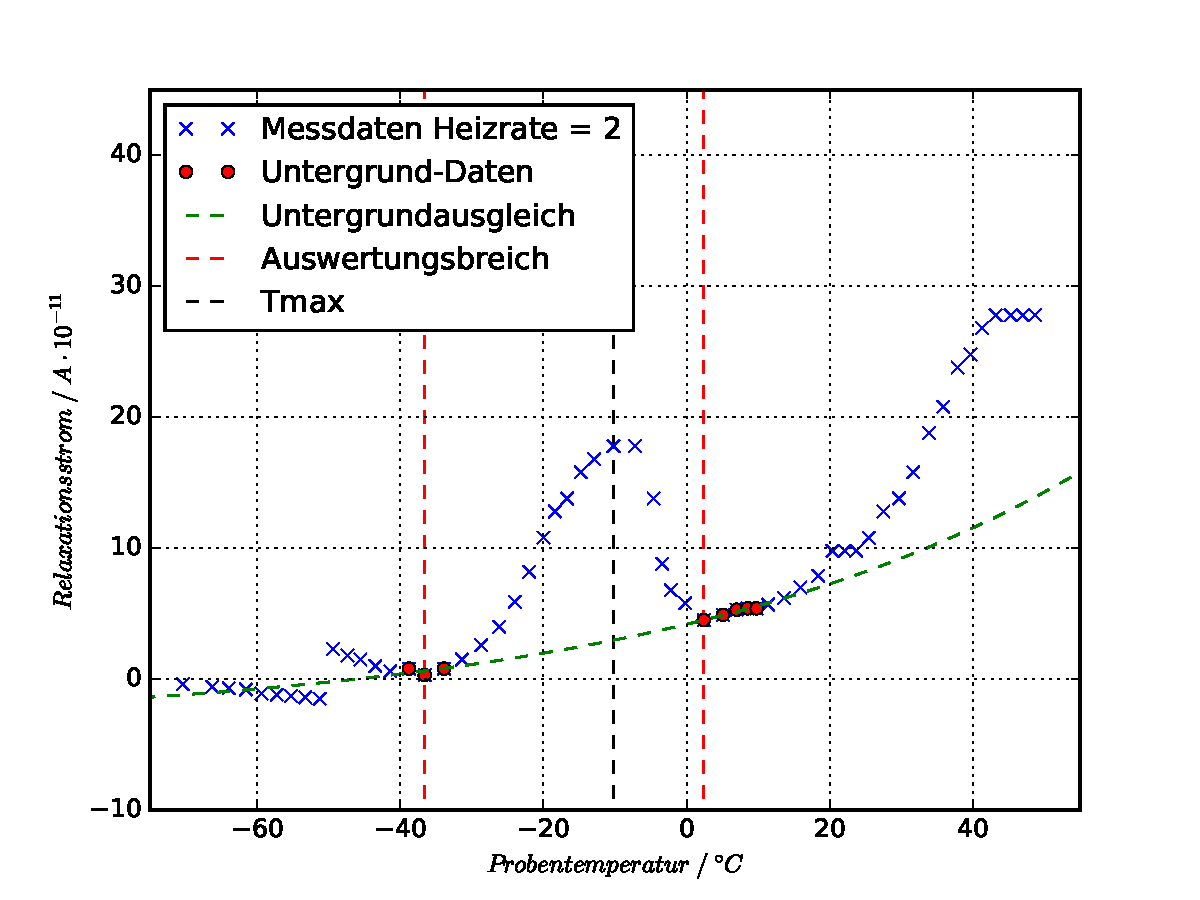
\includegraphics[height = 10cm]{plots/M1UGplot.pdf}
  \caption{Darstellung der Daten die mit Heizrate \SI{2}{\celsius\per\minute} aufgenommen wurden.}
  \label{fig:U2plot}
\end{figure}
\begin{figure}
  \centering
  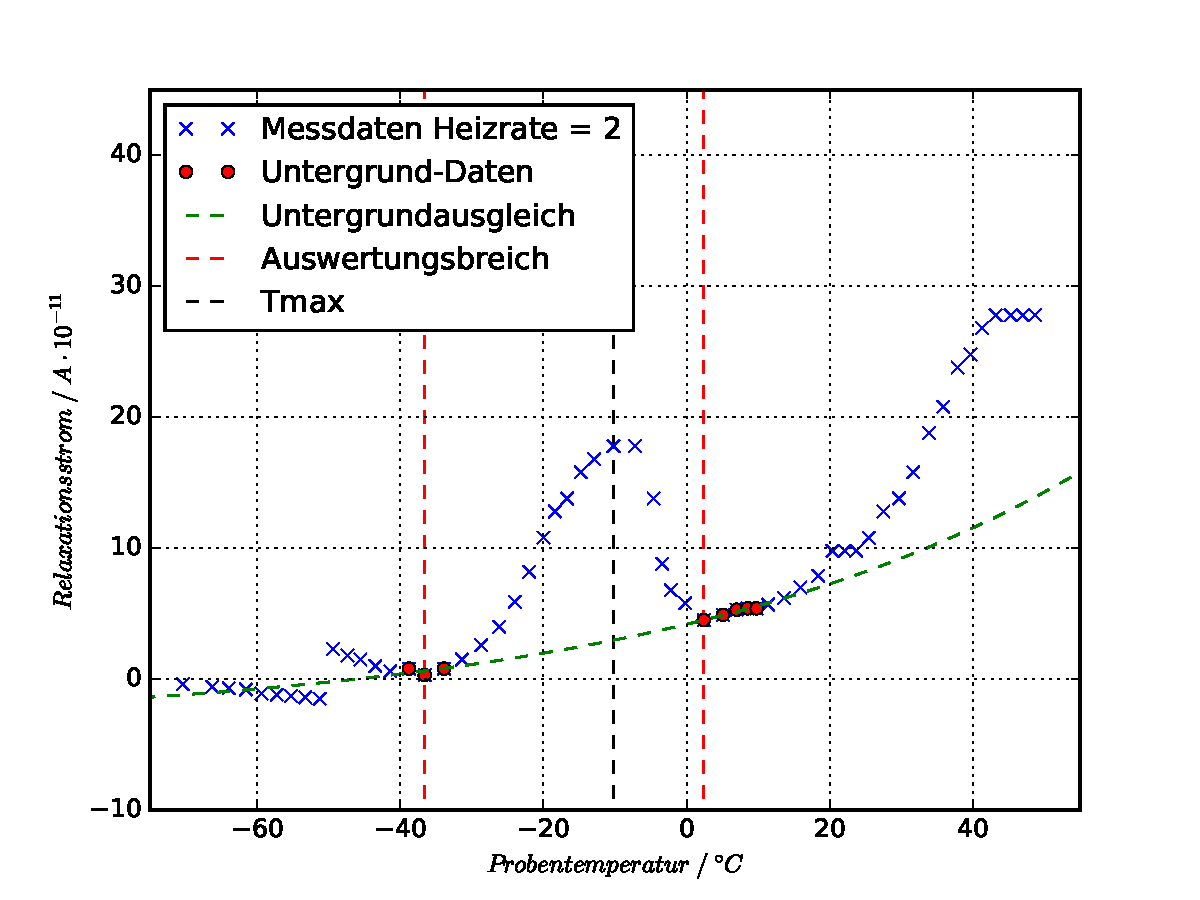
\includegraphics[height = 10cm]{plots/M1UGplot.pdf}
  \caption{Darstellung der Daten die mit Heizrate \SI{1.5}{\celsius\per\minute}aufgenommen wurden.}
  \label{fig:U15plot}
\end{figure}
\FloatBarrier
\paragraph{Bestimmung der Akivierungsenergie anhand der Nährung der Stromdichte}
Der folgende Teil der Auswertung bezieht sich auf die Nährung \eqref{eq:StromdichteNäherung2} 
der Stromdichte. Durch logarithmieren dieser Gleichung ergibt sich folgender Ausdruck:
\begin{equation}
\ln(i(T)) = - \frac{W}{kT} + const  = - A \cdot \frac{1}{T} + B	
\label{eq:lnfit}
\end{equation}
Dabei ist zu beachten, dass diese Nährung nur im Anfangsbereich der Kurve gültig ist. 
In dieser Auswertung wurden die Bereiche des ersten Minimums bis zum Maximums der Relaxationskurve 
verwendet, die in den Abbildungen \ref{fig:U2plot},\ref{fig:U15plot} zuvor eingezeichnet waren.   


\begin{figure}
  \centering
  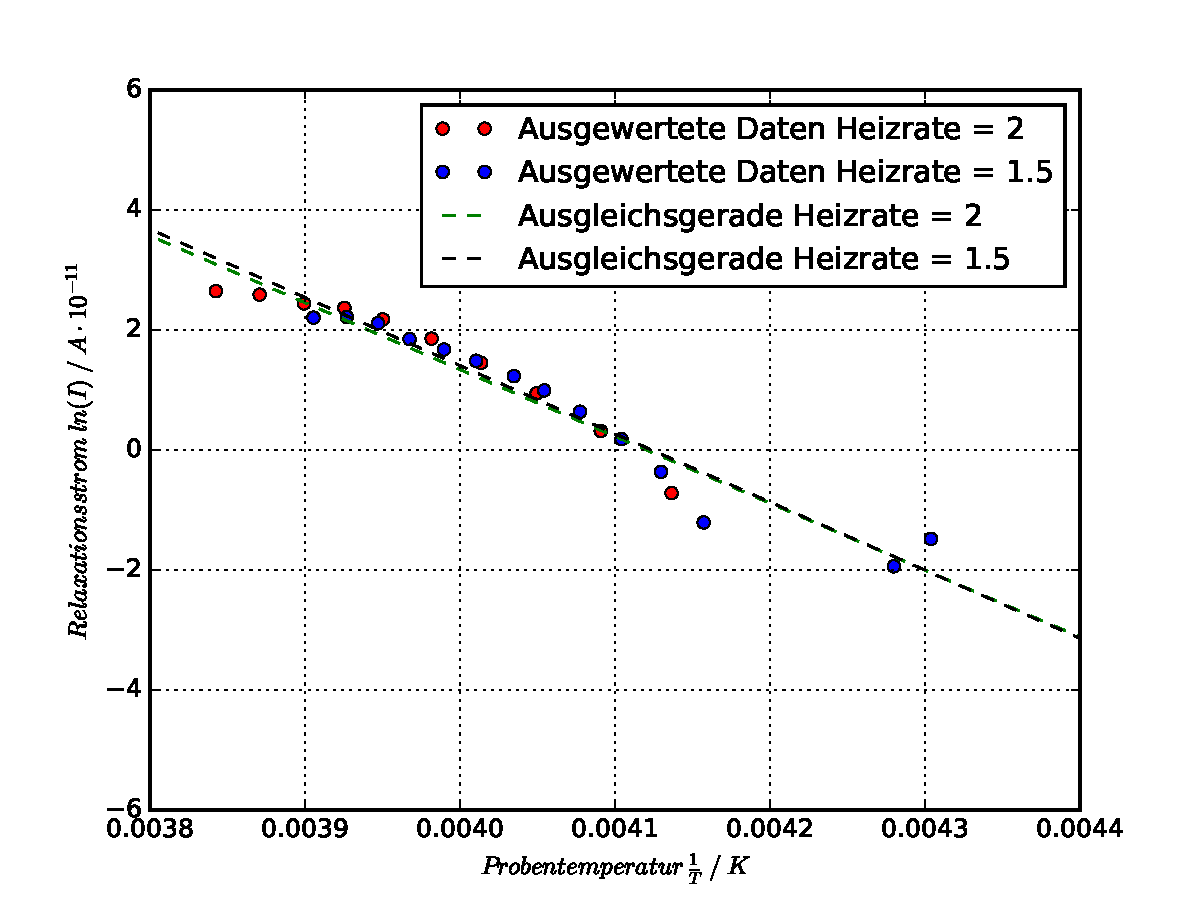
\includegraphics[height = 10cm]{plots/1.MethFitW.pdf}
  \caption{Darstellung der Datan im Gültigkeitsbereich der Nährung.}
  \label{fig:Meth1}
\end{figure}

